%!TEX TS-program = pdflatex
% dissertation.tex -- main dissertation file
%
% Wisconsin dissertation template
% Copyright (c) 2008-2009 William C. Benton.  All rights reserved.
%
% This program can redistributed and/or modified under the terms
% of the LaTeX Project Public License Distributed from CTAN
% archives in directory macros/latex/base/lppl.txt; either
% version 1 of the License, or (at your option) any later version.
%
% This program includes other software that is licensed under the
% terms of the LPPL and the Perl Artistic License; see README for details.
%
% You, the user, still hold the copyright to any document you produce
% with this software (like your dissertation).
%

%%% You'll want ``oneside'' for the deposit version, but probably not for any versions that don't need to meet the UW requirements
\documentclass[12pt,oneside,letterpaper]{memoir}


% preamble.tex -- packages to include
%
% Wisconsin dissertation template
% Copyright (c) 2008 William C. Benton.  All rights reserved.
%
% This program can redistributed and/or modified under the terms
% of the LaTeX Project Public License Distributed from CTAN
% archives in directory macros/latex/base/lppl.txt; either
% version 1 of the License, or (at your option) any later version.
%
% This program includes other software that is licensed under the
% terms of the LPPL and the Perl Artistic License; see README for details.
%
% You, the user, still hold the copyright to any document you produce
% with this software (like your dissertation).

%% You should use natbib
\IfFileExists{natbib.sty}{%
\usepackage{natbib}%
}{}

%% You probably need appendix, if you want appendices
\IfFileExists{appendix.sty}{%
\usepackage{appendix}%
}{}

%% the spacing in memoir is weird, you'll need to use this
\DisemulatePackage{setspace}
\usepackage[onehalfspacing]{setspace}

%% List setup; the ``hanglist`` environment will allow you to have
%% nicely-typeset enumerated lists (i.e. with the numbers hanging in
%% the margins).  You need at least version 2.1 of enumitem.sty.  If
%% you don't have enumitem installed at all, hanglist will just be an
%% alias for enumerate.
\IfFileExists{enumitem.sty}{%
\usepackage[loadonly]{enumitem}[2007/06/30]%
\newlist{hanglist}{enumerate}{1}% 
\setlist[hanglist]{label=\arabic*.}%
\setlist[hanglist,1]{leftmargin=0pt}%
}{%
\newenvironment{hanglist}{\begin{enumerate}}{\end{enumerate}}%
}

%% Comment out any of these that you don't want
\usepackage{amssymb}
\usepackage{amsmath}
\usepackage{amsthm}
%\usepackage{theorem}
\usepackage{hyperref}

\usepackage{outline}

\IfFileExists{mathpartir.sty}{%
\usepackage{mathpartir}%
}{}

%%%%% LISTINGS package and setup
\IfFileExists{listings.sty}{%
\usepackage{listings}%
}{}



%% Get rid of ugly borders around PDF hyperlinks (e.g. for cross-references, bib entries, or URLs)
\hypersetup{pdfborder = 0 0 0}

%% You want microtype.
\IfFileExists{microtype.sty}{%
\usepackage[protrusion=true,expansion=true]{microtype}%
}{}

%\pagestyle{thesisdraft}

% Surround parts of graphics with box
\usepackage{boxedminipage}

%% booktabs (thx to Nate Rosenblum for bringing this beautiful package
%% to my attention)
\IfFileExists{booktabs.sty}{%
\usepackage{booktabs}%
}{}

% This is now the recommended way for checking for PDFLaTeX:
\usepackage{ifpdf}

%% Avoid ugly "Type 3" fonts
\usepackage{lmodern}
\usepackage[LY1]{fontenc}

%% Substitute your favorite serif and sans fonts here....
\IfFileExists{tgpagella.sty}{%
% TeX Gyre pagella, like Palatino
\usepackage{tgpagella}%
}{}

\usepackage[LY1]{eulervm}

\ifpdf
\usepackage[pdftex]{graphicx}
\else
\usepackage{graphicx}
\fi

\usepackage{makeidx}
\makeindex

{\theoremstyle{plain}
\newtheorem{thm}{Theorem}[chapter]
\newtheorem{cor}[thm]{Corollary}
\newtheorem{define}[thm]{Definition}
\newtheorem{exmpl}[thm]{Example}
}
{\theoremstyle{remark}
\newtheorem{rmk}[thm]{Remark}
}

\newtheoremstyle{customsty1}
{3pt}%
{3pt}%
{}% --- body font
{}% --- indent amount
{\bfseries}% --- Theorem head font
{:}% --- Punctuation after head
{.5em}% --- space after head
{}% --- theorem head spec (can be left empty, meaning 'normal')

% Define 'newtheorems' that use ``customsty1''
{\theoremstyle{customsty1} 
}


%%% NB: the ``deposit'' chapter- and page- styles should conform to UW
%%% requirements.  If you are producing a pretty version of your
%%% dissertation for web use later, you will certainly want to make
%%% your own chapter and page styles.

\makechapterstyle{deposit}{%
  \renewcommand{\chapterheadstart}{}
  \renewcommand{\printchaptername}{}
  \renewcommand{\chapternamenum}{}
  \renewcommand{\printchapternum}{\parbox{2em}{\MakeLowercase{\Large\scshape\thechapter{}}} }
  \renewcommand{\afterchapternum}{}
  \renewcommand{\printchaptertitle}[1]{%
  \raggedright\Large\scshape\MakeLowercase{##1}}
  \renewcommand{\afterchaptertitle}{%
  \vskip\onelineskip \hrule\vskip\onelineskip}
}

\makepagestyle{deposit}
 
\makeatletter
 
\renewcommand{\chaptermark}[1]{\markboth{#1}{}}
\renewcommand{\sectionmark}[1]{\markboth{#1}{}}
 
\makeevenfoot{deposit}{}{}{}
\makeoddfoot{deposit}{}{}{}
\makeevenhead{deposit}{\thepage}{}{}
\makeoddhead{deposit}{}{}{\thepage}
\makeatother

%%% set up page numbering for chapter pages to satisfy UW requirements
%%% NB: You will want to delete until the ``SNIP'' mark if you are
%%% making a ``nice'' copy
\copypagestyle{chapter}{plain}
\makeoddfoot{chapter}{}{}{}
\makeevenhead{chapter}{\thepage}{}{}
\makeoddhead{chapter}{}{}{\thepage}
%%% SNIP

%%% bib nonsense
\makeatletter
\newenvironment{wb-bib}[1]{%
  \chapter*{references}
\ifnobibintoc\else 
\phantomsection 
\addcontentsline{toc}{chapter}{References} 
\fi 
\prebibhook
  \begin{bibitemlist}{#1}}{\end{bibitemlist}\postbibhook}

\AtBeginDocument{%
  \@ifpackageloaded{natbib}{% natbib is loaded
    \addtodef{\endthebibliography}{}{\vskip-\lastskip\postbibhook}
    \@ifpackagewith{natbib}{sectionbib}{% with sectionbib option
      \renewcommand{\bibsection}{\@memb@bsec}}%
      {\renewcommand{\bibsection}{\@memb@bchap}}}%
  {}
  \@ifpackagewith{chapterbib}{sectionbib}{%
    \renewcommand{\sectionbib}[2]{}
    \renewcommand{\bibsection}{\@memb@bsec}}{}
}
\makeatother

% defs.tex -- wbepi environment for chapter epigraphs and other useful defs.
%
% Wisconsin dissertation template
% Copyright (c) 2008 William C. Benton.  All rights reserved.
%
% This program can redistributed and/or modified under the terms
% of the LaTeX Project Public License Distributed from CTAN
% archives in directory macros/latex/base/lppl.txt; either
% version 1 of the License, or (at your option) any later version.
%
% This program includes other software that is licensed under the
% terms of the LPPL and the Perl Artistic License; see README for details.
%
% You, the user, still hold the copyright to any document you produce
% with this software (like your dissertation).


%% put lstnewenvironment declarations here, if you're using listings

%% end lstnewenvironment declarations

%% I put convenience definitions that will go in several chapters here

%%%%% begin convenience definitions

\makeatletter
\newcommand{\wb@episource}{}
\newenvironment{wbepi}[1]{\begin{quote}\renewcommand{\wb@episource}{#1}\itshape}{\par\upshape \raggedleft --- \textsc{\wb@episource}\\ \end{quote}}
\makeatother

%%%%% SVN
\IfFileExists{svn-multi.sty}{%
\usepackage{svn-multi}%
%%% Uncomment the second one and comment out the first one if you want
%%% to include subversion revision information in each file.
\newcommand{\vcinfo}{}%
%\newcommand{\vcinfo}{\begin{centering}\fbox{\fbox{\parbox{5in}{Author: \svnauthor\\Revision: \svnfilerev\\Last changed on: \svnfiledate\\URL: \svnkw{HeadURL}}}}\\[1em]\end{centering}}%
}{%
\newcommand{\svnidlong}[4]{}%
\newcommand{\svnfilerev}{}%
\newcommand{\svnauthor}{}%
\newcommand{\svnfiledate}{}%
\newcommand{\svnkw}{}%
\newcommand{\vcinfo}{}%
}

%%%%% end convenience definitions

% thesisdefs.tex

% This is mostly adapted from withesis.cls.  The original copyright
% notice for withesis.cls follows, preceded by two percent signs (%%):

%% withesis.cls
%% LaTeX Style file for the University of Wisconsin-Madison Thesis Format
%% Adapted from the Purdue University Thesis Format
%% Originally by Dave Kraynie
%% Edits by Darrell McCauley
%% Adapted to UW-Madison format by Eric Benedict  (Noted with <EB>)
%% Updated to LaTeX2e by Eric Benedict 24 July 00
%% 
%%=============================================================================
%% Licensed under the Perl Artistic License.
%% see: http://www.ctan.org/tex-archive/help/Catalogue/licenses.artistic.html
%% for more info...
%%=============================================================================

% withesis.cls is available from CTAN.  The modifications to this file
% are also licensed under the Perl Artistic License.

% --wb, 2008

\makeatletter

\newcounter {tocpage}
\newcounter {lofpage}
\newcounter {lotpage}
\newcounter {listofheading}

\newcommand\@thesistitlemedskip{0.2in}
\newcommand\@thesistitlebigskip{0.6in}
\newcommand{\degree}[1]{\gdef\@degree{#1}}
\newcommand{\project}{\gdef\@doctype{A masters project report}}
\newcommand{\prelim}{\gdef\@doctype{A preliminary report}}
\newcommand{\thesis}{\gdef\@doctype{A thesis}}
\newcommand{\dissertation}{\gdef\@doctype{A dissertation}}
\newcommand{\department}[1]{\gdef\@department{(#1)}}

\newenvironment{titlepage}
 {\@restonecolfalse\if@twocolumn\@restonecoltrue\onecolumn
  \else \newpage \fi \thispagestyle{empty}
% \c@page\z@ -- deleted: count title page in thesis
}{\if@restonecol\twocolumn \else \newpage \fi}

\gdef\@degree{Master of Science}    %Default is PhD
\gdef\@doctype{A thesis}         %Default is dissertation

\gdef\@department{(Engineering Physics)} % Default is Electical Engineering
\gdef\@defensedate{01/01/2100}% Default is a long time from now.
\gdef\@committee{
  Jane Doeverything, Professor, Electrical Engineering\\
  John Dosomethings, Associate Professor, Electrical Engineering\\
  }

\renewcommand{\maketitle}{%
  \begin{titlepage}
%-----------------------------------------------------------------------------
% -- The thesis office doesn't like thanks on title page.  Put it in
% -- the acknowledgments.  This is here so you don't have to change
% -- your titlepage when converting from report style. -> from Purdue, but I
%        left it here since it seems compatible with UW-Madison, Eric
%-----------------------------------------------------------------------------
    \def\thanks##1{\typeout{Warning: `thanks' deleted from thesis titlepage.}}
    \let\footnotesize\small \let\footnoterule\relax \setcounter{page}{1}
    \begin{center}
      {\textbf{\expandafter\expandafter{\@title}}} \\[\@thesistitlebigskip]
       by \\[\@thesistitlemedskip]
      \@author \\[\@thesistitlebigskip]
      \@doctype\ submitted in partial fulfillment of \\
      the requirements for the degree of\\[\@thesistitlebigskip]
      \@degree \\[\@thesistitlemedskip]
      \@department \\[\@thesistitlebigskip]
      at the \\[\@thesistitlemedskip]
      UNIVERSITY OF WISCONSIN--MADISON\\[\@thesistitlemedskip]
      \@date
    \end{center}
    \hspace*{-0.7in}Date of final oral examination: \@defensedate \\[\@thesistitlemedskip]
    \hspace*{-0.7in}The dissertation is approved by the following members of the 
    Final Oral Committee:\\
    \@committee
  \end{titlepage}
  \setcounter{footnote}{0}
  \setcounter{page}{1} %title page is NOT counted
  \let\thanks\relax
  \let\maketitle\relax \let\degree\relax \let\project\relax \let\prelim\relax
  \let\department\relax
  \gdef\@thanks{}\gdef\@degree{}\gdef\@doctype{}
  \gdef\@department{}
  %\gdef\@author{}\gdef\@title{}
}


%=============================================================================
% ABSTRACT
%=============================================================================
% The abstract should begin with two single-spaced lines describing
% the author and title in a standard format.  After these lines comes
% the standard abstract.
%=============================================================================
\def\abstract{
  \chapter*{Abstract}
  \addcontentsline{toc}{chapter}{Abstract}
  \relax\markboth{Abstract}{Abstract}}
\def\endabstract{\par\newpage}


%=============================================================================
% UMI ABSTRACT
%=============================================================================
% The UMI abstract should begin with the author and title in a standard format.
% After the author comes the advisor and university. After these lines comes
% a bunch of double spaced text to make up the standard abstract.
% After the abstract, the advisor's approval signature follows.
% This page is not numbered and is delivered seperately to the thesis office.
%=============================================================================

\def\advisortitle#1{\gdef\@advisortitle{#1}}
\def\advisorname#1{\gdef\@advisorname{#1}}
\gdef\@advisortitle{Professor}
\gdef\@advisorname{Cheer E.\ Place}

\def\umiabstract{
             \thispagestyle{empty}
                  \addtocounter{page}{-1}
                \begin{center}
                  {\textbf{\expandafter\uppercase\expandafter{\@title}}}\\
                  \vspace{12pt}
                  \@author \\
                  \vspace{12pt}
                  Under the supervision of \@advisortitle\ \@advisorname\\
                  At the University of Wisconsin-Madison
                \end{center}
}

\def\endumiabstract{\vfill \hfill\@advisorname\par\newpage}


%============================================================================
% VERBATIMFILE
%============================================================================
% \verbatimfile{<filename>}    for verbatim inclusion of a file
% - Note that the precise layout of line breaks in this file is important!
% - added the \singlespace - EB
%============================================================================
\def\verbatimfile#1{\begingroup \singlespace
                    \@verbatim \frenchspacing \@vobeyspaces
                    \input#1 \endgroup
}


%=============================================================================
% SEPARATOR Pages
%   Creates a blank page with a text centered horizontally and vertically.
%   The page is neither counted nor numbered.
%   These pages are required in the thesis format before sections such
%   as appendices, vita, bibliography, etc.
%=============================================================================
\def\separatorpage#1{
  \newpage
  \thispagestyle{empty}
  \addtocounter{page}{-1}
  \null
  \vfil\vfil
  \begin{center}
    {\textbf{#1}}
  \end{center}
  \vfil\vfil
  \newpage}


%=============================================================================
% COPYRIGHTPAGE
%=============================================================================
% The copyright must do the following:
% - start a new page with no number
% - place the copyright text centered at the bottom.
%=============================================================================
\def\copyrightpage{
  \newpage
  \thispagestyle{empty}    % No page number
  \addtocounter{page}{-1}
  \chapter*{}            % Required for \vfill to work
  \begin{center}
   \vfill
   \copyright\ Copyright by \@author\ \@date\\
   All Rights Reserved
  \end{center}}


%=============================================================================
% GLOSSARY
%=============================================================================
% The glossary environment must do the following:
% - produce the table of contents entry for the glossary
% - start a new page with GLOSSARY centered two inches from the top
%=============================================================================
\def\glossary{
  \chapter*{GLOSSARY}
  \addcontentsline{toc}{chapter}{Glossary}}
\def\endglossary{\par\newpage}

%=============================================================================
% NOMENCLATURE
%=============================================================================
% The nomenclature environment must do the following:
% - produce the table of contents entry for the nomenclature section
% - start a new page with NOMENCLATURE centered two inches from the top
%=============================================================================
\def\nomenclature{\separatorpage{DISCARD THIS PAGE}
  \chapter*{Nomenclature}
  \addcontentsline{toc}{chapter}{NOMENCLATURE}}
\def\endnomenclature{\par\newpage}

%=============================================================================
% CONVENTIONS
%=============================================================================
% The conventions environment must do the following:
% - produce the table of contents entry for the nomenclature section
% - start a new page with CONVENTIONS centered two inches from the top
%=============================================================================
\def\conventions{\separatorpage{DISCARD THIS PAGE}
  \chapter*{Conventions}
  \addcontentsline{toc}{chapter}{CONVENTIONS}}
\def\endconventions{\par\newpage}


%=============================================================================
% COLOPHON
%=============================================================================
% The colophon environment must do the following:
% - produce the table of contents entry for the nomenclature section
% - start a new page with COLOPHON centered two inches from the top
%=============================================================================
\def\colophon{\separatorpage{DISCARD THIS PAGE}
  \chapter*{Colophon}
  \addcontentsline{toc}{chapter}{Colophon}}
\def\endcolophon{\par\newpage}

%=============================================================================
% LIST OF SYMBOLS
%=============================================================================
% The list of symbols environment must do the following:
% - produce the table of contents entry for the list of symbols section
% - start a new page with LIST OF SYMBOLS centered two inches from the top
%=============================================================================
\def\listofsymbols{\separatorpage{DISCARD THIS PAGE}
  \eject
  \chapter*{LIST OF SYMBOLS}
  \addcontentsline{toc}{chapter}{LIST OF SYMBOLS}}
\def\endlistofsymbols{\par\newpage}

%=============================================================================
% VITA
%=============================================================================
% The vita environment must do the following:
% - produce a separator page with the word vita centered
% - produce the table of contents entry for the vita
% - start a new page with VITA centered two inches from the top
%=============================================================================
\def\vita{
%  \separatorpage{VITA}         % UW doesn't require this EB
  \chapter*{VITA}
  \addcontentsline{toc}{chapter}{VITA}}
\def\endvita{\par\newpage}

%=============================================================================
% ACKNOWLEDGMENTS
%=============================================================================
% The acknowledgments environment must do the following:
% - start a new page with ACKNOWLEDGMENTS centered two inches from the top
%=============================================================================
\def\acks{
  \chapter*{Acknowledgments}
}
\def\endacks{\par\newpage}

%=============================================================================
% DEDICATION
%=============================================================================
% The dedication environment must do the following:
% - start a new page
% - center the text vertically
% - include the text in a center environment
%=============================================================================
\def\dedication{
  \newpage
  \null\vfil
  \begin{center}}
\def\enddedication{\end{center}\par\vfil\newpage}

%=============================================================================
% DATE
%=============================================================================
%\def\today{\ifcase\month\or
  %January\or February\or March\or April\or May\or June\or
  %July\or August\or September\or October\or November\or December\fi
  %\space\number\day, \number\year}
\newcount\@testday
\def\today{\@testday=\day
  \ifnum\@testday>30 \advance\@testday by -30
  \else\ifnum\@testday>20 \advance\@testday by -20
  \fi\fi
  \number\day\ \
  \ifcase\month\or
    January \or February \or March \or April \or May \or June \or
    July \or August \or September \or October \or November \or December
    \fi\ \number\year
}


%  Single counter for theorems and theorem-like environments:
\newtheorem{theorem}{Theorem}[chapter]
\newtheorem{assertion}[theorem]{Assertion}
\newtheorem{claim}[theorem]{Claim}
\newtheorem{conjecture}[theorem]{Conjecture}
\newtheorem{corollary}[theorem]{Corollary}
\newtheorem{definition}[theorem]{Definition}
\newtheorem{example}[theorem]{Example}
\newtheorem{figger}[theorem]{Figure}
\newtheorem{lemma}[theorem]{Lemma}
\newtheorem{prop}[theorem]{Proposition}
\newtheorem{remark}[theorem]{Remark}

%=============================================================================
% TABLE OF CONTENTS; LIST OF FIGURES; LIST OF TABLES
%=============================================================================
% In report style, \tableofcontents, \listoffigures, etc. are always
% set in single-column style.  @restonecol is used to keep track of
% whether we need to switch back to double column style after the toc.
%
% The only known problem now is that the first page with the new
% layout is too long.  The problem seems to be that the change to
% textheight doesn't take place on the first page.  Even if it's the
% first line in the table of contents macro.  Presumably the same
% problem also occurs in the lof and lot.
%
% I'm taking a shot at fixing the problem by dropping in a throw-away
% page between the change to the height parameters and the start of
% the chapter.  Isn't elegance wonderful?
%
%=============================================================================

% \def\@tableof#1#2#3#4#5{
% { % limit scope of following declarations!!
%   \@restonecolfalse\if@twocolumn\@restonecoltrue\onecolumn\fi
%   \addtolength{\textheight}{-40pt}       % -24-16
%   \addtolength{\majorheadskip}{-40pt}    % -24-16
%   \addtolength{\headheight}{52pt}        %  36+16
%   \addtolength{\headsep}{-12pt}          % -12
%   \separatorpage{DISCARD THIS PAGE}
%   \chapter*{#1}
%   #5
%   \relax\markboth{#1}{#1}
%   \hbox to \hsize{#2 \hfil Page}
%   \singlespace
%   \setcounter{#3}{0}
%   \setcounter{listofheading}{1}  % change from 0 to 1 by mccauley, 14may93
%   \def\@oddhead{\vbox to \headheight{\vspace{4pt}
%     \hbox to \hsize{\hfil\textrm{\thepage}} \vfil
%     \ifnum\value{#3}=1
%       \ifnum\value{listofheading}=2
%         \hbox to \hsize{Appendix\hfil} \vspace{4pt} \fi
%       \ifnum\value{listofheading}=1
%         \stepcounter{listofheading} \fi
%       \hbox to \hsize{#2 \hfil Page}
%     \else
%       \setcounter{#3}{1}
%     \fi}}
%   \def\@evenhead{\vbox to \headheight{\vspace{4pt}
%     \hbox to \hsize{\textrm{\thepage}\hfil} \vfil
%     \ifnum\value{#3}=1
%       \ifnum\value{listofheading}=2
%         \hbox to \hsize{Appendix\hfil} \vspace{4pt} \fi
%       \ifnum\value{listofheading}=1
%         \stepcounter{listofheading} \fi
%       \hbox to \hsize{#2 \hfil Page}
%     \else
%       \setcounter{#3}{1}
%     \fi}}
%   \@starttoc{#4}  \if@restonecol\twocolumn\fi
%   \newpage
% }}
% 
% \def\tableofcontents{\@tableof{TABLE OF CONTENTS}{}{tocpage}{toc}{}}
% 
% \def\listoffigures{
%   \@tableof{LIST OF FIGURES}{Figure}{lofpage}{lof}
%   {\protect\addcontentsline{toc}{chapter}{LIST OF FIGURES}}}
% 
% \def\listoftables{
%   \@tableof{LIST OF TABLES}{Table}{lotpage}{lot}
%   {\protect\addcontentsline{toc}{chapter}{LIST OF TABLES}}}

%=============================================================================
% BIBLIOGRAPHY
%=============================================================================
% The thebibliography environment executes the following commands:
%
%  o start a new 'chapter' with BIBLIOGRAPHY as the heading
%  o produce a separator page for the bibliography
%
%  \def\newblock{\hskip .11em plus .33em minus -.07em} --
%      Defines the `closed' format, where the blocks (major units of
%      information) of an entry run together.
%
%  \sloppy  -- Used because it's rather hard to do line breaks in
%      bibliographies,
%
%  \sfcode`\.=1000\relax --
%      Causes a `.' (period) not to produce an end-of-sentence space.
%=============================================================================
% \altbibtitle
%   The default title for the References chapter is ``LIST OF REFERENCES''
%   Since some people prefer ``BIBLIOGRAPHY'', the command
%   \altbibtitle has been added to change the chapter title.
%   This command does nothing more than change REFERENCES to BIBLIOGRAPHY
%============================================================================
\def\@bibchaptitle{Bibliography}
\def\altbibtitle{\def\@bibchaptitle{Bibliography}}
\def\thebibliography#1{
  %\separatorpage{\@bibchaptitle}
  \global\@bibpresenttrue
  \chapter*{\@bibchaptitle\markboth{\@bibchaptitle}{\@bibchaptitle}}
  \addcontentsline{toc}{chapter}{\@bibchaptitle}
  \vspace{0.375in}    % added to match 4 line requirement
  \interlinepenalty=10000 % added to prevent breaking of bib entries
  \singlespace\list
  {[\arabic{enumi}]}{\settowidth\labelwidth{[#1]}\leftmargin\labelwidth
    \advance\leftmargin\labelsep \usecounter{enumi}}
  \def\newblock{\hskip .11em plus .33em minus -.07em}
  \sloppy
  \sfcode`\.=1000\relax}
\let\endthebibliography=\endlist



\makeatother



\clearpage\pagenumbering{roman}  % This makes the page numbers Roman (i, ii, etc)

\newcommand{\keff}{k$_{eff}$ }
\newcommand{\uran}{$^{235}$U }
\newcommand{\pu}{$^{238}$Pu }


\title{Surrogate Reactor Modeling for Space Electrical System Mass Optimization}
\author{Alexander Swenson}
\department{Nuclear Engineering, Engineering Physics}

\date{2018}

\begin{document}

%%% Uncomment the following if your .bib contains references that you will not 
%%% explicitly cite, but that should be in the final bibliography:
% \nocite{*}

\ifpdf
\DeclareGraphicsExtensions{.pdf, .jpg, .tif}
\else
\DeclareGraphicsExtensions{.eps, .jpg}
\fi

\maketitle


%% Add \part declarations if you want, but it's not necessary
%\part{Preliminaries}

\svnidlong{$LastChangedBy$}{$LastChangedRevision$}{$LastChangedDate$}{$HeadURL: http://freevariable.com/dissertation/branches/diss-template/frontmatter/frontmatter.tex $}
\vcinfo{}

%%% SOME OF THIS CODE IS ADAPTED FROM THE VENERABLE withesis.cls

% COPYRIGHT PAGE
%  - To include a copyright page use \copyrightpage
\copyrightpage

% DEDICATION
\begin{dedication}
	\emph{Please insert your dedication here.}
\end{dedication}

%% BEGIN PAGESTYLE

%%% You can pick a pagestyle if you want; see the memoir class
%%% documentation for more info.  The default ``deposit'' option meets
%%% the UW thesis typesetting requirements but is probably
%%% unsatisfactory for making a version of your dissertation that
%%% won't be deposited to the graduate school (e.g. for web or a nice
%%% printed copy)

\chapterstyle{deposit}
\pagestyle{deposit}


% ACKNOWLEDGMENTS
\begin{acks}
This project was funded by the Department of Energy's Nuclear Energy University
Program. I am grateful for the financial support that allowed me to conduct my
research. In addition to our project sponsors, I have many others to thank for their
support over the years.

I owe Dr. Paul Wilson a immense amount of gratitude for his years of continued
academic support and guidance. You are the embodiment of what it means to be
a researcher, and educator, and a citizen. Your dedication to the well-being of your
students is something we should all aspire to. I can say with absolute
certainty that I would not be in the position I am today without your help. 
Thank you for advising me as a student in the Computational Nuclear Engineering 
Research Group (CNERG). My experience working with you has been nothing short of phenomenal.

I would like to thank Dr. Greg Nellis for his support of my work. You have
been an invalueable resource to me on this project. Your advice and patience was
incredibly helpful as I worked out the kinks in my thermal hydraulic model. I
also owe a thanks to Becky Sondelski, the graduate student responsible for the
power cycle model development. I am thankful to have had the opportunity to work with you.

I would also like to thank my colleagues in CNERG. Thank you Young-Hui Park 
for taking me in as an undergraduate researcher assisting on your project
and for helping me to be the graduate researcher I am today. Thank you
Pat Shriwise and Baptiste Mouginot for your friendship and countless hours of
banter and laughter, it made the hard days a little less so. Thank you Katie
Mummah and Katie Biegel, I will forever cherish our camaraderie as we navigated
our first year of grad school together. Thank you Chelsea D'Angelo and Nancy
Granda-Duarte for your long conversations and commiserations in 434, I will be
forever grateful for our friendships. Every day on the fourth floor of ERB 
was a new adventure-both personally and professionally, to everyone in CNERG,
your consistent positive attitudes and support made working here a privilege. I
will always view our academic and professional relationships as overshadowed by
our personal friendships. I will miss this community dearly.

To the students, faculty, and staff, both past and present of the Engineering
Physics Department, thank you for making this a safe and enjoyable place to
learn and work. I have spent nearly 6 years as a member of this community and I
will cherish every moment for the rest of my life. The friendships and
professional connections I have made in my time here will continue to fulfill me
as I move on with my career. We have a truly special program and
an even better community here. While I look forward to my next challenges, 
I will mourn the loss of this community in my daily life.

To my friend Sam Rebenstorf. Your friendship has been a relief from 
my academic frustrations over my entire time at UW. Thank you for being there
for me and supporting me as I worked towards my Master's degree.

To my sisters Libby and Mary. Thank you for your consistent cheerleading and
love over the years. Your company has always been a respite from the struggles
and monotony of everyday life. I learn so much from you both and can't express
how happy I am to be your brother.

To my parents Andy and Patty, thank you for your support, love, and guidance for
the past 24 years. You raised me to think for myself, to always stay curious,
and to never give up. I will always appreciate the sacrifices you made for 
Libby, Mary, and me.

Finally I would like to thank my girlfriend, Julia. Your companionship meant
the world to me as I fumbled my way through grad school. You have been
a steady source of support and comfort in my life and I could not be luckier
than I am with you. You provide me with constant motivation to push 
boundaries and become the best possible version of myself. 
I cannot wait to see what we accomplish together.

\end{acks}

% CONTENTS, TABLES, FIGURES
\renewcommand{\printtoctitle}[1]{\chapter*{#1}}
\renewcommand{\printloftitle}[1]{\chapter*{#1}}
\renewcommand{\printlottitle}[1]{\chapter*{#1}}

\renewcommand{\tocmark}{}
\renewcommand{\lofmark}{}
\renewcommand{\lotmark}{}

\renewcommand{\tocheadstart}{}
\renewcommand{\lofheadstart}{}
\renewcommand{\lotheadstart}{}

\renewcommand{\aftertoctitle}{}
\renewcommand{\afterloftitle}{}
\renewcommand{\afterlottitle}{}

\renewcommand{\cftchapterfont}{\normalfont} 
\renewcommand{\cftsectionfont}{\itshape} 
\renewcommand{\cftchapterpagefont}{\normalfont} 
\renewcommand{\cftchapterpresnum}{\bfseries} 
\renewcommand{\cftchapterleader}{} 
\renewcommand{\cftsectionleader}{} 
\renewcommand{\cftchapterafterpnum}{\cftparfillskip} 
\renewcommand{\cftsectionafterpnum}{\cftparfillskip} 

% \captionnamefont{\small\sffamily} 
% \captiontitlefont{\small\sffamily} 

% \renewcommand{\contentsname}{contents}
% \renewcommand{\listfigurename}{list of figures}
% \renewcommand{\listtablename}{list of tables}

\tableofcontents

\clearpage
\listoftables

\clearpage
\listoffigures

\clearpage
% NOMENCLATURE
% \begin{conventions}
% % \begin{description}
% % \item{\makebox[0.75in][l]{term}
% %        \parbox[t]{5in}{definition\\}}
% % \end{description}
% \input{conventions}
% \end{conventions}

%% The UW graduate school no longer wants a UMI abstract page
%% Should you need one for some reason, uncomment the following
%% lines.  Thanks to Matt Fredrikson for reporting this!

% \advisorname{Gottlob Frege}
% \advisortitle{Professor}
% \begin{umiabstract}
%  \textbf{FIXME:  basically a placeholder; do not believe}

\svnidlong{$LastChangedBy$}{$LastChangedRevision$}{$LastChangedDate$}{$HeadURL: http://freevariable.com/dissertation/branches/diss-template/frontmatter/abstract.tex $}
\vcinfo{}

I did some research, read a bunch of papers, published a couple myself, (pick one):
\begin{enumerate}
	\item ran some experiments and made some graphs,
	\item proved some theorems
\end{enumerate}
and now I have a job.  I've assembled this document in the last couple of months so you will let me leave.  Thanks!
% \end{umiabstract}

\begin{abstract}
  \textbf{FIXME:  basically a placeholder; do not believe}

\svnidlong{$LastChangedBy$}{$LastChangedRevision$}{$LastChangedDate$}{$HeadURL: http://freevariable.com/dissertation/branches/diss-template/frontmatter/abstract.tex $}
\vcinfo{}

I did some research, read a bunch of papers, published a couple myself, (pick one):
\begin{enumerate}
	\item ran some experiments and made some graphs,
	\item proved some theorems
\end{enumerate}
and now I have a job.  I've assembled this document in the last couple of months so you will let me leave.  Thanks!
\end{abstract}

\clearpage\pagenumbering{arabic}

%%% END STUFF TAKEN FROM WITHESIS EXAMPLE FILE


%% Now include the tex files for each chapter, like so (I put these in separate dirs): 
\chapter{Background and Project Description}
Electrical power is vital for NASA to achieve its deep space exploration goals.
Electricity powers life support systems for astronaut habitats, communication
with Earth, and allows astronauts to perform experiments to help us better
understand the solar system. Long-life, high-output, compact electrical power
systems are vital to achieving future space exploration goals. Launch costs 
often restrict the design of systems launched
into space, currently NASA is under contract with SpaceX to deliver supplies to
the International Space Station (ISS) in low-earth orbit (LEO). SpaceX delivers
supplies to the ISS for more that \$55,000 per kg. Launch costs to Mars or the
Moon will be significantly higher given the required energy to escape Earth
orbit. As a consequence, when designing a terrestrial electrical system for
solar system exploration, it is crucial to minimize the mass of the system. This
work was a sub-set of a larger
project to explore the mass tradeoff between the critical components of the
electrical power system in order to minimize the mass of the system as a whole.
This project developed the reactor mass model to support the goal of the overall
project.

\section{Scope}
The purpose of this work was not to develop a fully-fledged reactor concept.
High-fidelity core modeling of neutronics and thermal hydraulics was not
performed for this work.
This project focused on exploring the tradeoffs between reactor mass and the
mass of significant components of the power cycle. Traditional reactor physics
tools could not be used for depletion calculations because they are to slow to
integrate into an optmization routine. To support the optimization effort, this project focused on
developing a surrogate model for the reactor mass to be integrated into the
power cycle model. This model needed to take inputs from the power cycle and
rapidly exceute to return the minimum mass reactor that could meet the thermal
power requirement of the power cycle. The overall cycle was constrained to the
target lifetime and power outputs dictated by the project sponsors. The reactor
was modeled sufficiently such that future work could feasibly develop the
concept into a deployable reactor within a reasonable amount of time.

\section{Constraints}
The two main constraints for the system were provided by the project sponsors,
and ultimately dictated by NASA. NASA has identified the following performance
requirements: a 10 year lifetime and a 40 kWe power level, as sufficient to
support future terrestrial exploration throughout the solar system. All fuel
options were available for the reactor with a preferance for high near-term
technical readiness. High enriched uranium is acceptable. The reactor will be direct-cooled and coupled to a
supercritical carbon dioxide brayton cycle to produce the desired electrical
output. The reactor will be used only for terrestrial applications, not in
transit. This helps shielding mass, because the reactor can be buried prior to
startup.

\section{Previous Space Reactor Work}
Using nuclear technology to power space systems is not a new concept. Various
space programs have been using nuclear technology for decades to power
statellites and deep space probes. Generally, nuclear power systems for space
exploration can be grouped into two categories, Radioisotope Thermoelectric
Generators (RTGs) and Fission Power Systems (FPS). 

\subsection{Radioisotope Thermoelectric Generators}
Traditionally, NASA has relied on Radioisotope Thermoelectric Generators to
produce electricity for deep-space and long term exploration missions. These
devices produce power for spacecraft traveling far from the sun, to parts of the
solar system where they could not rely on solar panels to meet their electrical
needs. Since 1961, NASA has deployed 46 RTGs on 27 different space missions
\citep{mmrtg_fact}.

One of the more common examples of a successful RTG design is the
General-Purpose Heat Source Radioisotope Thermoelectric Generator (GPHS-RTG).
GPHS-RTG relied on a \pu alpha source to generate heat. Modules of \pu
generators were stacked together for a combined thermal power of 4410 Wt. The
converter used silicon-germanium converter elements to produce 285 W of
electrical power at the beginning of mission (BOM).
\citep{bennett_mission_2006}. 

The GPHS-RTG design has been used on
numerous NASA deep space missions including; Galileo, Ulysses, New Horizons,
Cassini. All of the aforementioned spacecraft have had or continue to have
satisfactory power performance from their RTGs. \citep{bennett_mission_2006}.
In addition to the GPHS-RTG, NASA has used similar RTG designs for other
missions. The Apollo moon missions, Viking and Curiosity Mars missions, Voyager
and Pioneer deep space probes have all used RTG technology to power their
instruments and communication systems. The Voyager probes continue to function,
sending back data to Earth as they push into interstellar space
\citep{mmrtg_fact}.

NASA has experienced great success using RTGs to power deep space missions. Many
RTG systems deployed decades ago are still enabling deep space exploration
across the solar system. Despite their stellar performance record, RTGs are not
designed to provide large amounts of electrical power. The efficiency of RTGs is
too low for consideration at the 40 kWe level. In addition the US supply of \pu
is dwindling. NASA can't afford to use a \pu system at the 40 kWe level. As a
result, a fission power system was deemed appropriate for the project.

\subsection{Fission Power Systems}
Since RTGs have limited mass performance at high power levels, this project focused on designing a
fission power system to meet the mission requirements. Experience from past
fission designs was sought to help limit the design of the reactor. The choice
for fuel was based off of past designs. Some designs that were explored include;
SP-100, Kilopower, NTP and NEP concepts, and other solid-core design concepts.
    
\subsubsection{SP-100}
    SP-100 was a concept fission power system design part of the
    Strategic Defense Initiative (SDI) of the United States. SDI was a defense program started by
    President Ronald Reagan's administration to defend the United States against intercontinental
    ballistic missiles from the Soviet Union. The cornerstone of the program was orbital systems to
    intercept the missiles before they re-entered the atmosphere. These systems
    had large electrical power requirements motivating the SP-100 project
    \citep{sp100}.

    SP-100 was a fission reactor coupled to thermoelectric converters that
    generated 100 kWe. The reactor was cooled with liquid lithium. Uranium
    nitride was chosen over \uox for its higher uranium density to allow a lower
    overall fuel mass. Pin type fuel assemblies were chosen with Nb-1Zr/Re
    cladding. Extensive material testing and irradiation was performed to
    verify the performance of the chosen fuels. While SP-100 was never built, it
    was a good example of a mature design concept developed for similar power
    applications. The project was not only tailored to defense needs, peaceful
    space exploration missions were also considered within the scope of the
    project.

    \subsubsection{Kilopower}
    The Kilopower reactor is a near-term reactor prototype under development at Los
    Alamos National Laboratory. The reactor was designed to achieve Technical
    Readiness Level 5 by 2017 \citep{gibson_nasas_2017}. The Kilopower project is a
    stirling engine system driven by a heat-pipe cooled core. The UMo core was
    manufactured at the Y-12 National Security Complex from 93\%, High-Enriched
    Uranium (HEU). Kilopower is a relevant reference because it fills a similar 
    mission profile as the current project. NASA's target for Kilopower was a 1-10 kWe unit. 
    The core was successfully tested from November 2017 to March 2018 \citep{poston_krusty_2018}. During the
    tests, the UMo core was operated at 800 $\degree$C and 10 kWt power. While the
    cooling and power cycle systems differ from a direct-brayton cycle reactor, the
    Kilopower core design provided a good basis from which to design a direct-cooled
    fast reactor.

    \subsubsection { Nuclear Thermal Propulsion }

    Nuclear thermal propulsion (NTP) is a promising alternative to chemical rockets for
    deep space missions. Nuclear thermal rockets improve the efficiency of
    traditional chemical rockets to drastically decrease the travel time to planets
    in the solar system. NTP has been pursued by the United States Air Force
    (USAF) and NASA in the past to shorten journeys to Mars. 

    NTP works by heating a working fluid (hydrogen is most common) and
    accelerating it through a de Laval nozzle creating thrust. Chemical rockets
    heat the fluid through exothermic reactions. NTP engines rely on fission
    energy to heat the fluid. Using fission power as the thermal energy source means the engine does not require and
    oxidizing fuel to drive combustion.

    In order for NTP to be viable, it must achieve thrust-to-weight performance
    similar to chemical rockets. NTP achieves this with high temperatures, the
    higher the operating temperature, the more energy the working fluid absorbs
    and the greater specific impulse of the engine. Historically, the NERVA
    program focused on graphite-moderated cores \citep{webb_combined_2011}, but
    these reactors had poor material performance at high temperatures including
    cladding cracking. More recent work has used CERMET fuel to reach higher
    temperatures than previous designs. Uranium suspended in a tungsten matrix
    can be pressed into blocks with coolant channels and can achieve remarkable
    power densities (9.34 GW/m3) allowing for feasible NTP performance
    \citep{webb_combined_2011}.

    \subsubsection{DoD Microgrid Concept}
    The United States Department of Defense (DoD) is pursuing a small fission
    reactor to support remote military installations by providing electrical
    power. Forward Operating Bases (FOBs) often struggle to find a stable
    electrical power source and the Department of Energy has directed national
    labs to leverage nuclear technology to solve this problem. The military
    identified 1 MWe as an electrical power target for the concept design
    \citep{army_reactor_slides}.
    Engineers at Los Alamos National Laboratory with experience in small core
    design worked to design a small fission core to meet these power needs. The
    reactor core was cooled with heat pipes and connected to a brayton cycle for
    power conversion.

    A monolithic core design was chosen for this project. There are multiple
    specific options for the design including separated fuel and coolant
    channels with fuel in pin form. Another option used dispersed fuel in a
    composite block with coolant channels. These cores offer durability because
    the fuel is stronger in block form.

    These monolithic designs were a good reference for a space reactor fuel.
    The monolithic designs are compact, durable and simple. Similar core designs
    can be found in numerous fission space concepts, including the recently
    tested Kilopower core.

    \subsubsection{INL Megawatt Concept Reactor}
    The Center for Space Nuclear Research at Idaho National Laboratory pursued a
    mass optimization for a megawatt-scale fission power system coupled to a
    high temperature brayton conversion cycle. The reactor was designed to
    support nuclear electric propulsion (NEP). NEP uses electricity from a
    reactor to ionize and accelerate a gas. Ion thrusters are extremely
    efficient and can be used for long-duration space flight. The advantage of
    NEP systems is the decoupling of the energy source and the propellant,
    similar to nuclear thermal propulsion. This decoupling reduces the amount of
    propellant required for a given mission.
    
    The proposed reactor design was fueled with a tungsten uranium-mononitride
    CERMET fuel. Like the NTP designs, CERMET fuel was explored because of its
    high thermal conductivity. The working fluid and coolant was helium. The
    reactor mass model was a combination of thermal hydraulic equations and
    critical mass requirements. MCNP5 was used to determine how much fuel mass
    was required for a given coolant channel radius. The result of the thermal
    and neutronic modeling was a analytic fit for the requried reactor mass as a
    function of reactor thermal power. The model was a simple linear fit to
    thermal power and did not account for mass effects driven by changing flow
    conditions (temperature, pressure, etc.) \citep{webb_combined_2011}. 
    
    The goal of the INL concept was also to minimize the overall mass of the
    power system. In addition to a linear reactor mass model, the project
    developed simplified mass models for the power cycle components.
    The total optimization was performed by coupling the power cycle
    component mass models and exploring the tradeoffs between their performance
    and masses.

\section{Background Summary}
Since humans have pursued space exploration, there has been a large amount of design, 
testing, and deployment of nuclear technology for spaceflight. Traditionally
RTGs have been used for deep space probes and terrestrial landers. Fission power
systems are being pursued for larger power needs such as terrestrial bases and
propulsion. Varying fuel and coolant concepts have been considered for fission
systems. Promising designs are using monolithic fuels, citing their fission
product retention and resistance to thermal expansion. Some projects, like
Kilopower have focused on deploying a system as soon as possible, to this end,
the Kilopower reactor design has been successfully tested at full fission power.
Other designs, such as the concept at INL have focused on mass optimization with
their power cycles. This project will expand on the efforts of the work at INL.
The power cycle and the reactor mass model coupling will be enhanced to include
flow conditions. In addition to coupling improvements, the entire optimization
will be performed with super-critical carbon dioxide. Fuel choices for the
reactor model will be informed from past design experience.

\section{Neutronic Constraints}

A valid reactor design must meet certain neutronics constraints. The main
neutronics constraint is reactivity. The reactor must be able to sustain a chain
reaction from startup, to the final second of the 10 year lifetime. End of Life
(EOL) reactivity was the target metric for the neutronic design of the core. It
was important to determine which reactor parameters had the strongest impact on
EOL \keff. An n-dimensional sampling was performed to explore EOL \keff
dependence on various reactor parameters.

\subsection{Neutronics Parameters}
Homogeneous MCNP6.1 depletion models were used to analyze the EOL \keff response
to neutronics parameters (predictors). The core region was homogenized and
surrounded by a graphite reflector. A large set of 5-dimensional predictors and
EOL \keff results was produced to investigate the neutronics parameter space.
These predictors and their results helped develop an understanding of the
reactor response to important design and operational parameters. High Throughput
Computing capabilities at UW were used to perform 3901 depletion calculations
with MCNP6.1. Each model represents a unique sampling in every dimension using
the Latin Hypercube Sampling (LHS) technique. The LHS technique ensured even
sampling for every dimension. The sampled and fixed dimensions/parameters are
shown in Table \ref{tab:lhs_sweep_vars}.

\begin{table}[h]
  \centering
  \caption{Homogeneous Geometry and Depletion Parameters}
  \begin{tabular}{ll}
    \toprule
     Core Radius                		   & 10 - 50 [cm] \\
     Reflector Thickness				   & 15 [cm]\\
     Core Aspect Ratio					   & 1 [-] \\
     Coolant Channel Radius                & 0.5 - 1 [cm] \\
     Fuel Pitch to Coolant Channel D.      & 1.1-1.6 [-]\\
     Fuel Enrichment 					   & 20\% - 90\% $^{235}$U\\
     Thermal Power						   & 80-200 [kW]\\
     Fuel Temp  						   & 300 [K]\\
     Reactor Physics Code, Data			   & MCNP6.1, ENDF-7.2
  \end{tabular}
  \label{tab:lhs_sweep_vars}
\end{table}

\subsection{Neutronics Sampling Results}
The target metric for the neutronics sampling was an EOL \keff equal to one. In
order to determine the dependence of EOL \keff on each swept parameter in Table
\ref{tab:lhs_sweep_vars}, EOL \keff was plotted against the parameters.

\subsubsection{Thermal Power}
Initially, the result of greatest interest was the mass dependence on thermal
power because thermal power was the coupling parameter with the power cycle.
Figure \ref{fig:eol_keff_vs_power} shows the relationship between thermal power
and EOL \keff.

\begin{figure}[h]
    \centering
    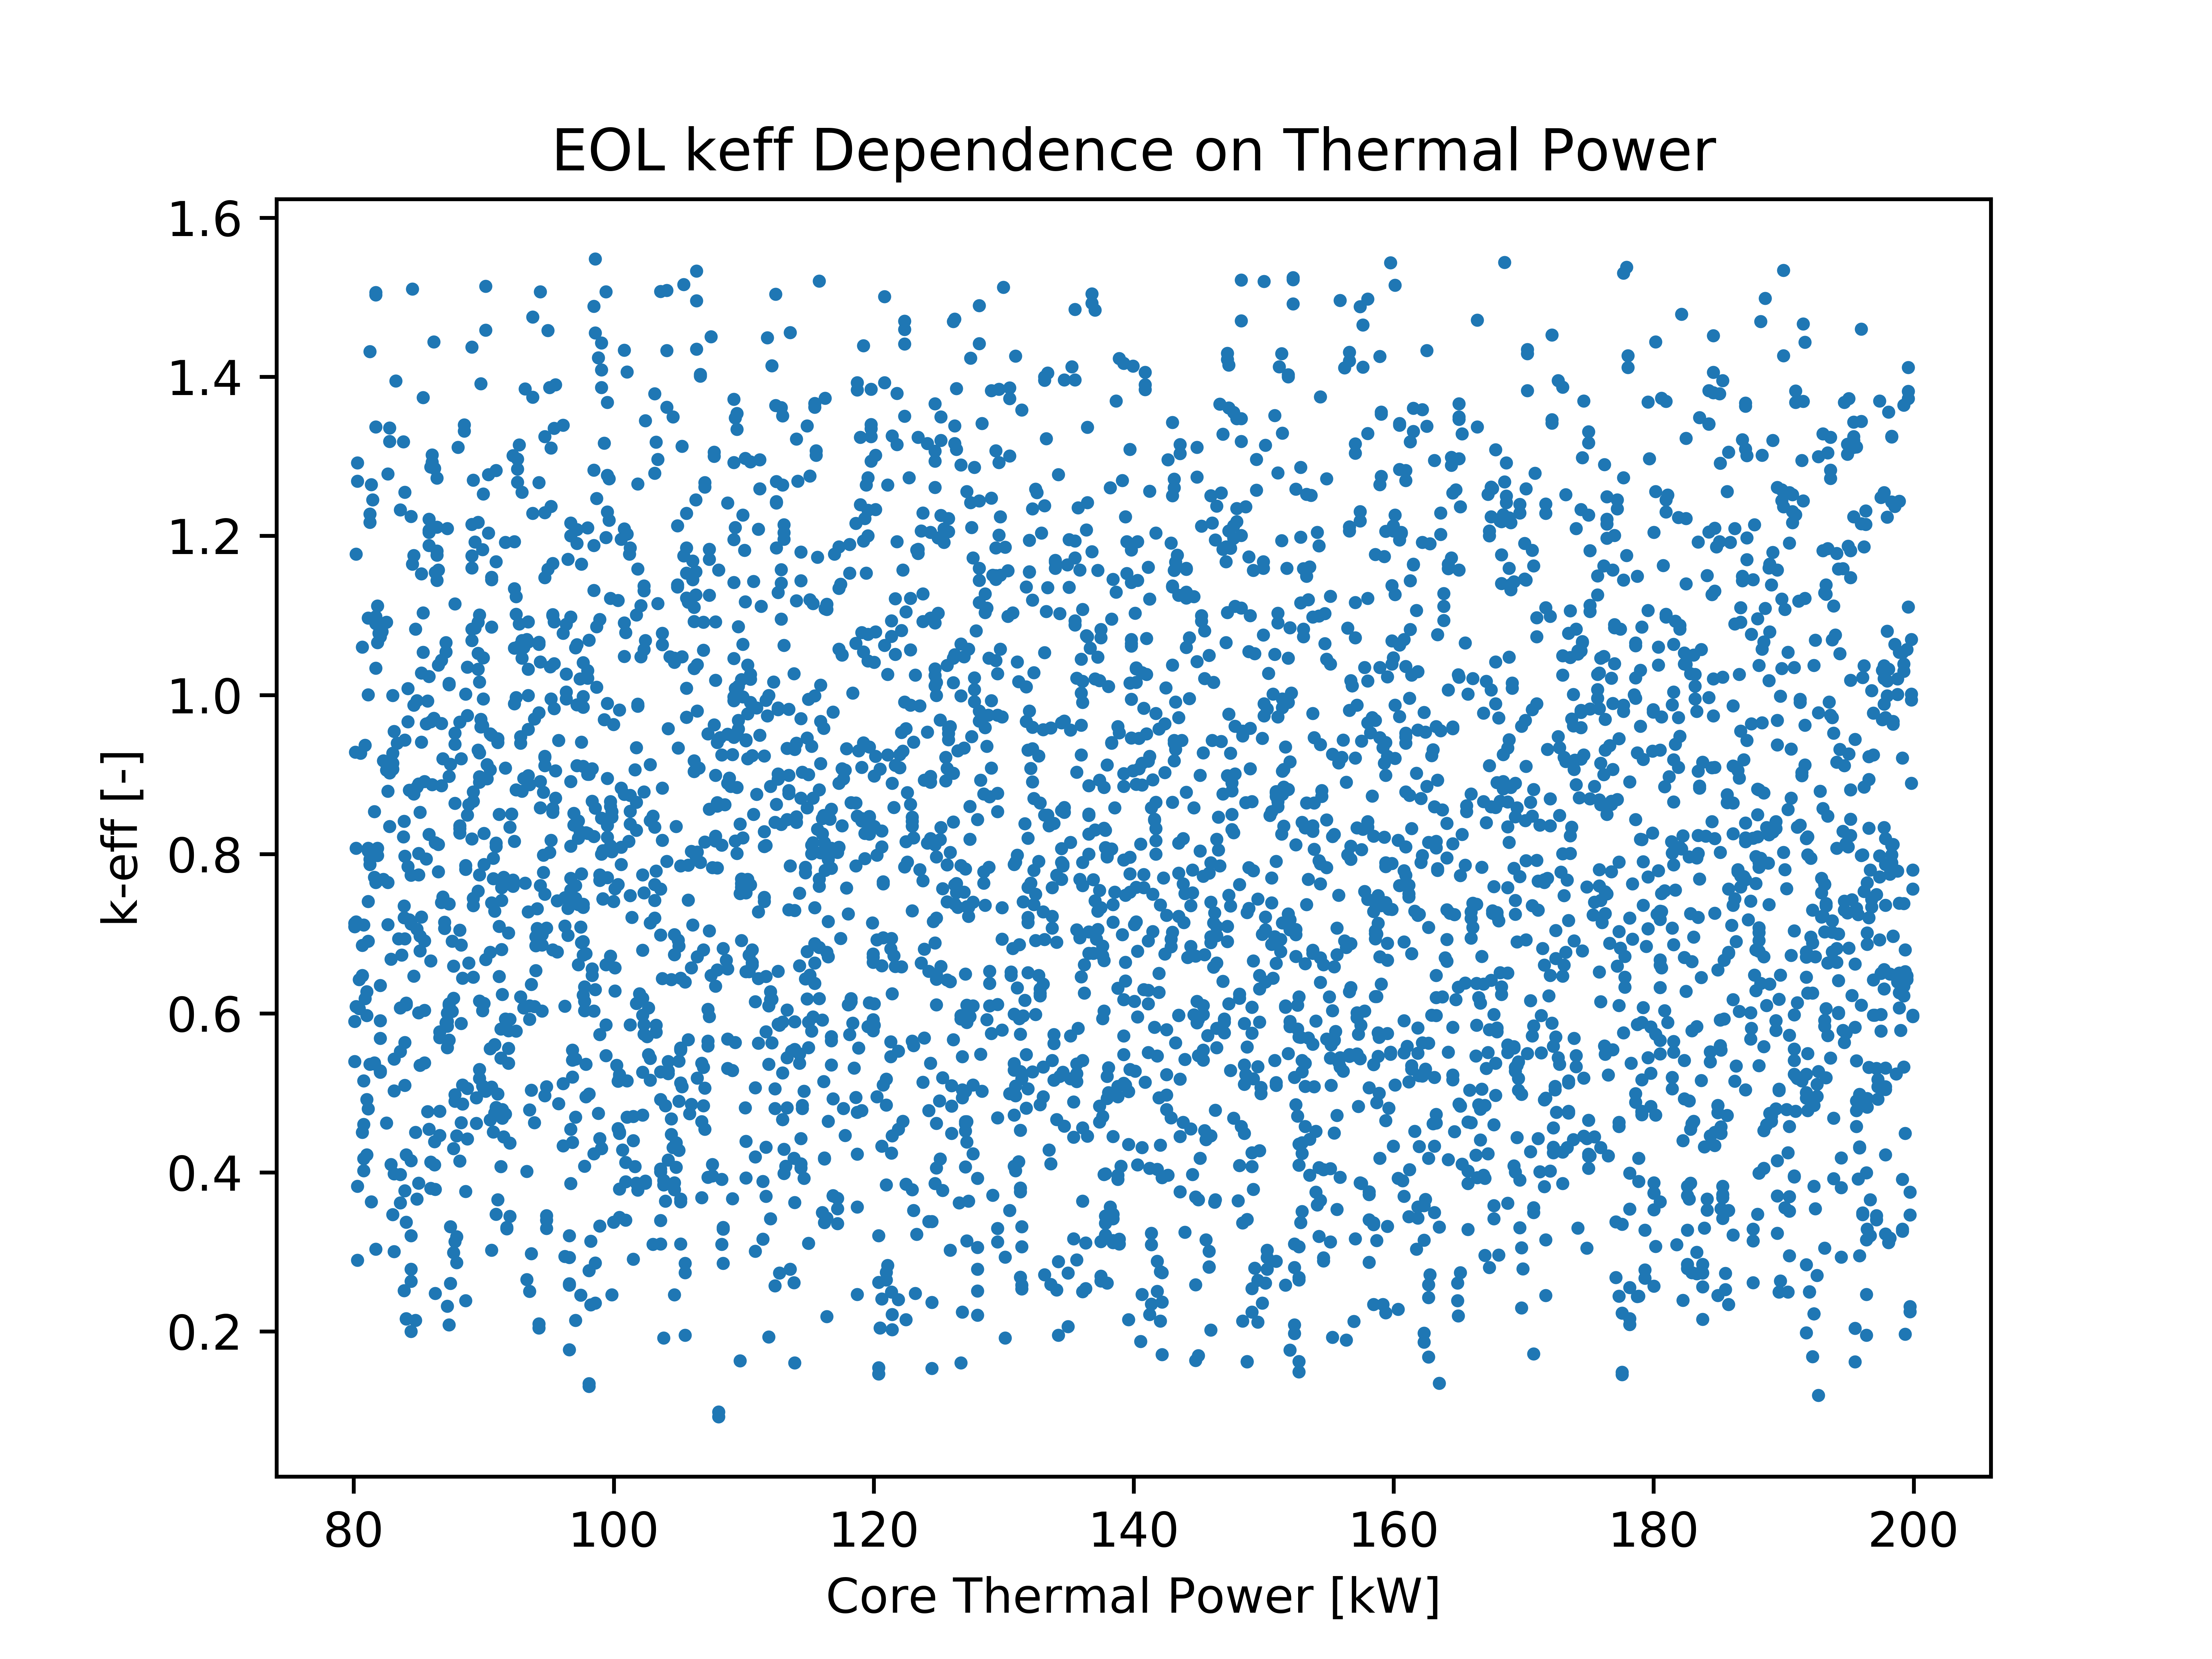
\includegraphics[width=3in]{nd_sweeps/keff_vs_power.png}
\caption{EOL \keff Power Dependence}
\label{fig:eol_keff_vs_power}
\end{figure}

As shown in Figure \ref{fig:eol_keff_vs_power}, EOL \keff is independent of core
thermal power. This result is not surprising considering the depletion rates in
the core. Assuming 1 MWd/gU is an achievable burnup, the reactor depletes
approximately 1000 kg of uranium at 200 kW of thermal power. The depletion mass
of uranium is negligigle compared to the mass of uranium required for the
reactor to be critical at BOL. Thermal power is not a strong predictor of EOL
criticality.

\subsubsection{Uranium 235 Mass}


\section{Reactor Mass Model} \label{reactor_mass_model}
The reactor mass model was created as a submodel of the power cycle mass
model. The reactor mass model was designed to take flow property inputs (T, P,
$\dot{m}$) and constrain a reactor concept that is both coolable, and critical
after 10 years of full power operation. The attribute of interest is the mass of
the valid concept, but other useful values such as geometry, fuel fraction,
and fluid-flow paramters are available from the solver. Before the mass model
could be built, some important design decisions needed to be made.

\subsection{Initial Design Constraints}
    In order to develop a reactor mass model, the concept was constrained with
some general design decisions. The chosen design needed to be simple and robust. The simplest reactor fuel concept is block fuel with coolant channels. 
Block fuel is a common design choice for space reactors that operate at relatively 
low power and burnup compared to power reactors. Two fuel types were chosen; one for
near-term and the other for long-term technological readiness options. Uranium
oxide was chosen as the near-term fuel option for its high melting temperature.
UMo and UN fuel were not considered because of tempearture limitations, despite
their thermal conductivity and uranium density advantages. Inconel-718 was
chosen as cladding for its high temperature strength and corrosion
compatability with sCO$_2$. With these design choices, the reactor mass model
could be developed from first principle heat transfer and fluid flow equations
coupled with a critical core radius constraint.

\subsubsection{Fuel Composition}
Two reactor fuels were considered for modeling. The near term technical
readiness choice was 93\% enriched \uox. The advanced fuel option investigated
was uranium-tungsten cermet (UW). UW-cermet fuel is UN fuel suspended in a
tungsten matrix. UW-cermet fuel has been considered for nuclear thermal
propulsion due to its high thermal conductivity and resistance to fuel swelling.
The tradeoff with UW-cermet fuel is a reduced uranium density, 60\% of the fuel
volume is UN, 40\% is tungsten. As shown below in Table \ref{tab:uox_comp} and
Table \ref{tab:uw_comp}, the \uox fuel has a significantly higher uranium
density than the UW-CERMET fuel.

\begin{table}[h]
  \centering
  \caption{\uox fuel composition}
  \begin{tabular}{cc}
    \toprule
    Isotope   & Mass Fraction [-] \\
    \midrule
     8016     & 0.1520 \\
    92235     & 0.7886 \\
    92238     & 0.0594 \\
  \end{tabular}
  \label{tab:uox_comp}
\end{table}
    
\begin{table}[h]
  \centering
  \caption{UW-CERMET fuel composition}
  \begin{tabular}{cc}
    \toprule
    Isotope   & Mass Fraction [-] \\
    \midrule
     7015     &  0.0260 \\
     74180    &  0.0006 \\ 
     74182    &  0.1396 \\
     74183    &  0.0758 \\
     74184    &  0.1632 \\
     74186    &  0.1531 \\
     92235    &  0.4107 \\
     92238    &  0.0309 \\
  \end{tabular}
  \label{tab:uw_comp}
\end{table}

\subsubsection{Fuel Design Modularity}
A fuel design was chosen to constraint the reactor model. In order to support
alternate designs, the reactor model was developed in a modular fashion.
Different fuel configurations such as pin-type or TRISO particle fuel could be
explored with a different set of heat transfer equations and criticality models.
This will be discussed in more detail in following sections.

\subsection{Thermal Hydraulic Theory}
    The first major constraint of a valid reactor design was coolability. The reactor must
not melt and the integrity of the fuel must be maintained for the duration of
the mission. To ensure the thermal hydraulic validity of a chosen design, 
    1D heat transfer and bulk-averaged fluid flow calculations were performed. The 1D
heat transfer and fluid equations were coupled with analytical flux shape
factors from nuclear engineering literature to determine the maximum extractable
thermal power for each reactor design. A 1D resistance network is used to
determine the maximum thermal generation for a given core design and temperature
drop between fuel meat and coolant.

\subsubsection{Flow Properties}
All flow properties were axially averaged between their inlet and outlet values.
The inlet and outlet flow conditions, thermal power, and mass flow rate are
dictated by the power cycle configuration and requirements. Property tables for
both CO2 and H2O coolants as a function of perssure and temperature were 
generated using EES and interpolated using SciPy's 2D interpolation functions.
The interpolated properties included: thermal conductivity, density, viscosity,
and specific heat.

\subsubsection{Core Geometry}

Important core geometry parameters were calculated. The coolant flow area,
average distance of conduction in the fuel, volume fraction of cladding in
coolant, number of coolant channels, convection surface area, LD, and the cross
sectional area for conduction in the fuel. The core radius is set by a critical
radius constraint dependent on the fuel fraction. This will be discussed in a
later section.

Fuel area and volume is derived from the core radius and fuel fraction. Where
$AR$ is the core aspect ratio.

\begin{equation}
    A_{fuel} = frac_{fuel}*r_{core}^2*\pi
\end{equation}
\begin{equation}
    V_{fuel} = A_{cool}*AR*r_{core}
\end{equation}

The fraction of cladding in the coolant is derived from the coolant channel
radius and cladding thickness.

\begin{equation}
    frac_{clad} = \frac{(r_{channel} + t_{clad})^2 - r_{channel}^2}{r_{channel}^2} 
\end{equation}

In a similar vein, coolant flow area is derived from the core radius, cladding
fraction, and fuel fraction

\begin{equation}
    A_{cool} = (1-frac_{fuel})*(1-frac_{clad})*r_{core}^2*\pi
\end{equation}

\begin{equation}
    V_{cool} = A_{cool}*AR*r_{core}
\end{equation}

The number of coolant channels is derived from the area of each channel and the
core flow area.

\begin{equation}
    N_{channels} = \frac{A_{cool}}{(r_{channel} + t_{clad})^2 * \pi}
\end{equation}

The convection surface area is dervied from the channel radius, core length, and
number of channels.

\begin{equation}
    A_{conv} = 2*r_{channel}*\pi*r_{core}*AR*N_{channels}    
\end{equation}

The length over diameter is derived from the channel radius and core length.

\begin{equation}
    LD = \frac{r_{core}*AR}{2*r_{channel}}
\end{equation}

The average distance to conduction is derived from fuel area and number of
channels.

\begin{equation}
    R_{cond} = \frac{\sqrt{\frac{A_{fuel}}{N_{channels}}}}{2}
    \label{r_cond}
\end{equation}

The cross sectional area for conduction in the fuel was conservatively estimated
as the convection surface area. In reality, the cross-sectional area changes as
heat transfers from the center of the fuel meat to the coolant channels.


These are the important equations defining the 1D geometry for a coolable
reactor. Once the geometry has been defined, the flow conditions are modeled.

\subsubsection{Flow Equations}

Once the core geometry has been defined, the flow is characterized using
bulk-averaged flow conditions and the reactor geometry. The mass flux, coolant
velocity, Reynold's number, Nusselt number and average heat transfer
coefficients are calculated.

Mass flux is derived from flow area and the mass flow rate dictated by the power
cycle. Flow velocity can be calculate from mass flux and density.

\begin{equation}
    \dot{G} = \frac{\dot{m}}{A_{flow}}
\end{equation}

\begin{equation}
    v = \frac{\dot{G}}{\rho}
\end{equation}

The Reynold's number is derived from flow velocity, density, viscosity, and the
characteristic flow length (channel diameter, D).

\begin{equation}
    Re = \frac{\rho v D}{\mu}
\end{equation}

The Nusselt number is calculated using the same correlations as EES. Laminar,
turbulent, and transitional flows are all treated differently.

The average heat transfer coefficient is derived from the Nusselt number and
thermal conductivity of the fluid.

\begin{equation}
    \bar{h} = \frac{Nu k_{cool}}{D}
\end{equation}

\subsubsection{1D Thermal Generation Modeling}

With a fully defined geometry and fully characterized flow, the maximum thermal
output of the core is calculated. The maximum generation (at the center of the
core) is calculated using a 1D resistance network. The three resistances in the
network are: conduction in the fuel, conduction in the clad, and convection from
the clad to the coolant. Gap and interface resistances were ignored.

Resistance to conduction in the fuel was approximated as plane wall conduction.
\begin{equation}
    R_{fuel} =  \frac{R_{cond}}{k_{fuel}A_{cond}}
\end{equation}

\begin{equation}
    R_{clad} = log(1+\frac{t_{clad}}{r_{channel}})
\end{equation}

\begin{equation}
    R_{conv} = \frac{1}{2\bar{h}r_{channel}L\pi N_{channels}}
\end{equation}

The maximum heat transfer rate at the fuel centerline was derived from the
resistance network and the temperature drop. The temperature drop was determined
by the maximum fuel temperature (estimated to be half the melting temperature of
the fuel) and the bulk coolant temperature.

\begin{equation}
    Q^{'''}_{max} = \frac{dT}{R_{fuel} + R_{clad} + R_{conv}}
\end{equation}

Finally, the thermal generation at fuel centerline is scaled by the axial and
radial flux profiles to account for the cosine and bessel function shapes of the
flux. The scaling factor was taken from El-Wakil's Nuclear Heat Transport.

\begin{equation}
    Q_{gen} = Q^{'''}_{max} * 0.275
\end{equation}

\subsubsection{1D Thermal Hydraulic Calcuations}

    The governing equations above describe a coolable
reactor design. A Python code was written to solve the system of equations
defining the geometry, flow conditions, and 1D heat transfer in the reactor. The
code utilizes Scipy's optimization package. The 'optimize\_scalar' function is
used to guess fuel fraction values. For each fuel fraction, the above equations
are used to determine $Q_{gen}$, an error exists between $Q_{gen}$ and the
required thermal reactor output dictated by the power cycle requirements. The
optimization function minimizes the squared difference between $Q_{gen}$ and the
thermal power requirements. When the solver converges on a fuel fraction, the
code returns a coolable reactor design. Since the core radius was set by a
critical radius constraint, this reactor is also neutronically valid for the
duration of the 10 year mission.
    The thermal hydrauilc code also calculates the mass of each reactor. This
mass includes fuel, cladding, coolant, reflector material and the pressure
vessel. The pressure vessel thickness was calculated as a function of pressure
and outer core radius (including the reflector) for stainless steel at \~700K.

%% etc, etc.

%% Do you have appendices?  If so, add them here, just like chapters.
% \begin{appendices}
% \include{backmatter/appendix1}
% \end{appendices}

%% Are you a big nerd with a colophon?  Add it here.
\begin{colophon}
\svnidlong{$LastChangedBy$}{$LastChangedRevision$}{$LastChangedDate$}{$HeadURL: http://freevariable.com/dissertation/trunk/frontmatter.tex $}
\vcinfo{}

This template uses Gyre Pagella by default.  (I used Arno Pro in my dissertation.)

Feel free to give me a shout-out in your colophon or acks if this template is useful for you.  Good luck!

\end{colophon}


%% McBride is a very nice style (some version is included in this distribution)
\bibliographystyle{mcbride}
\bibliography{bibliography}

%% Want an index?  Neither did I.
%\printindex

\end{document}
